% Indicate the main file. Must go at the beginning of the file.
% !TEX root = ../main.tex

%----------------------------------------------------------------------------------------
% CHAPTER TEMPLATE
%----------------------------------------------------------------------------------------


\chapter{Discussion and Outlook} % Main chapter title

\label{Chapter5} % Change X to a consecutive number; for referencing this chapter elsewhere, use \ref{ChapterX}

%----------------------------------------------------------------------------------------
% SECTION 1
%----------------------------------------------------------------------------------------

\section{Limits on simulation data driven approaches}

\subsection{Overfitting}
% missing the perfect simulation parameters --> deep learning approach!
Using simulated data as training data is an approach which intrinsically needs to be questioned. Under the assumption that the simulation approach used is accurate enough to explain the effects under investigation, we could argue that this effectively solves the task. However, this almost never holds for complex tasks such as ours and thus we expect overfitting on the experimental data.
The process of learning the domain gap between simulated and experimental spectra is commonly referred to as learning the domain shift. To visualize this, Figure \ref{fig:overfit} shows how the loss increases after 50 epochs of training. 

\begin{figure}[H]
    \centering
    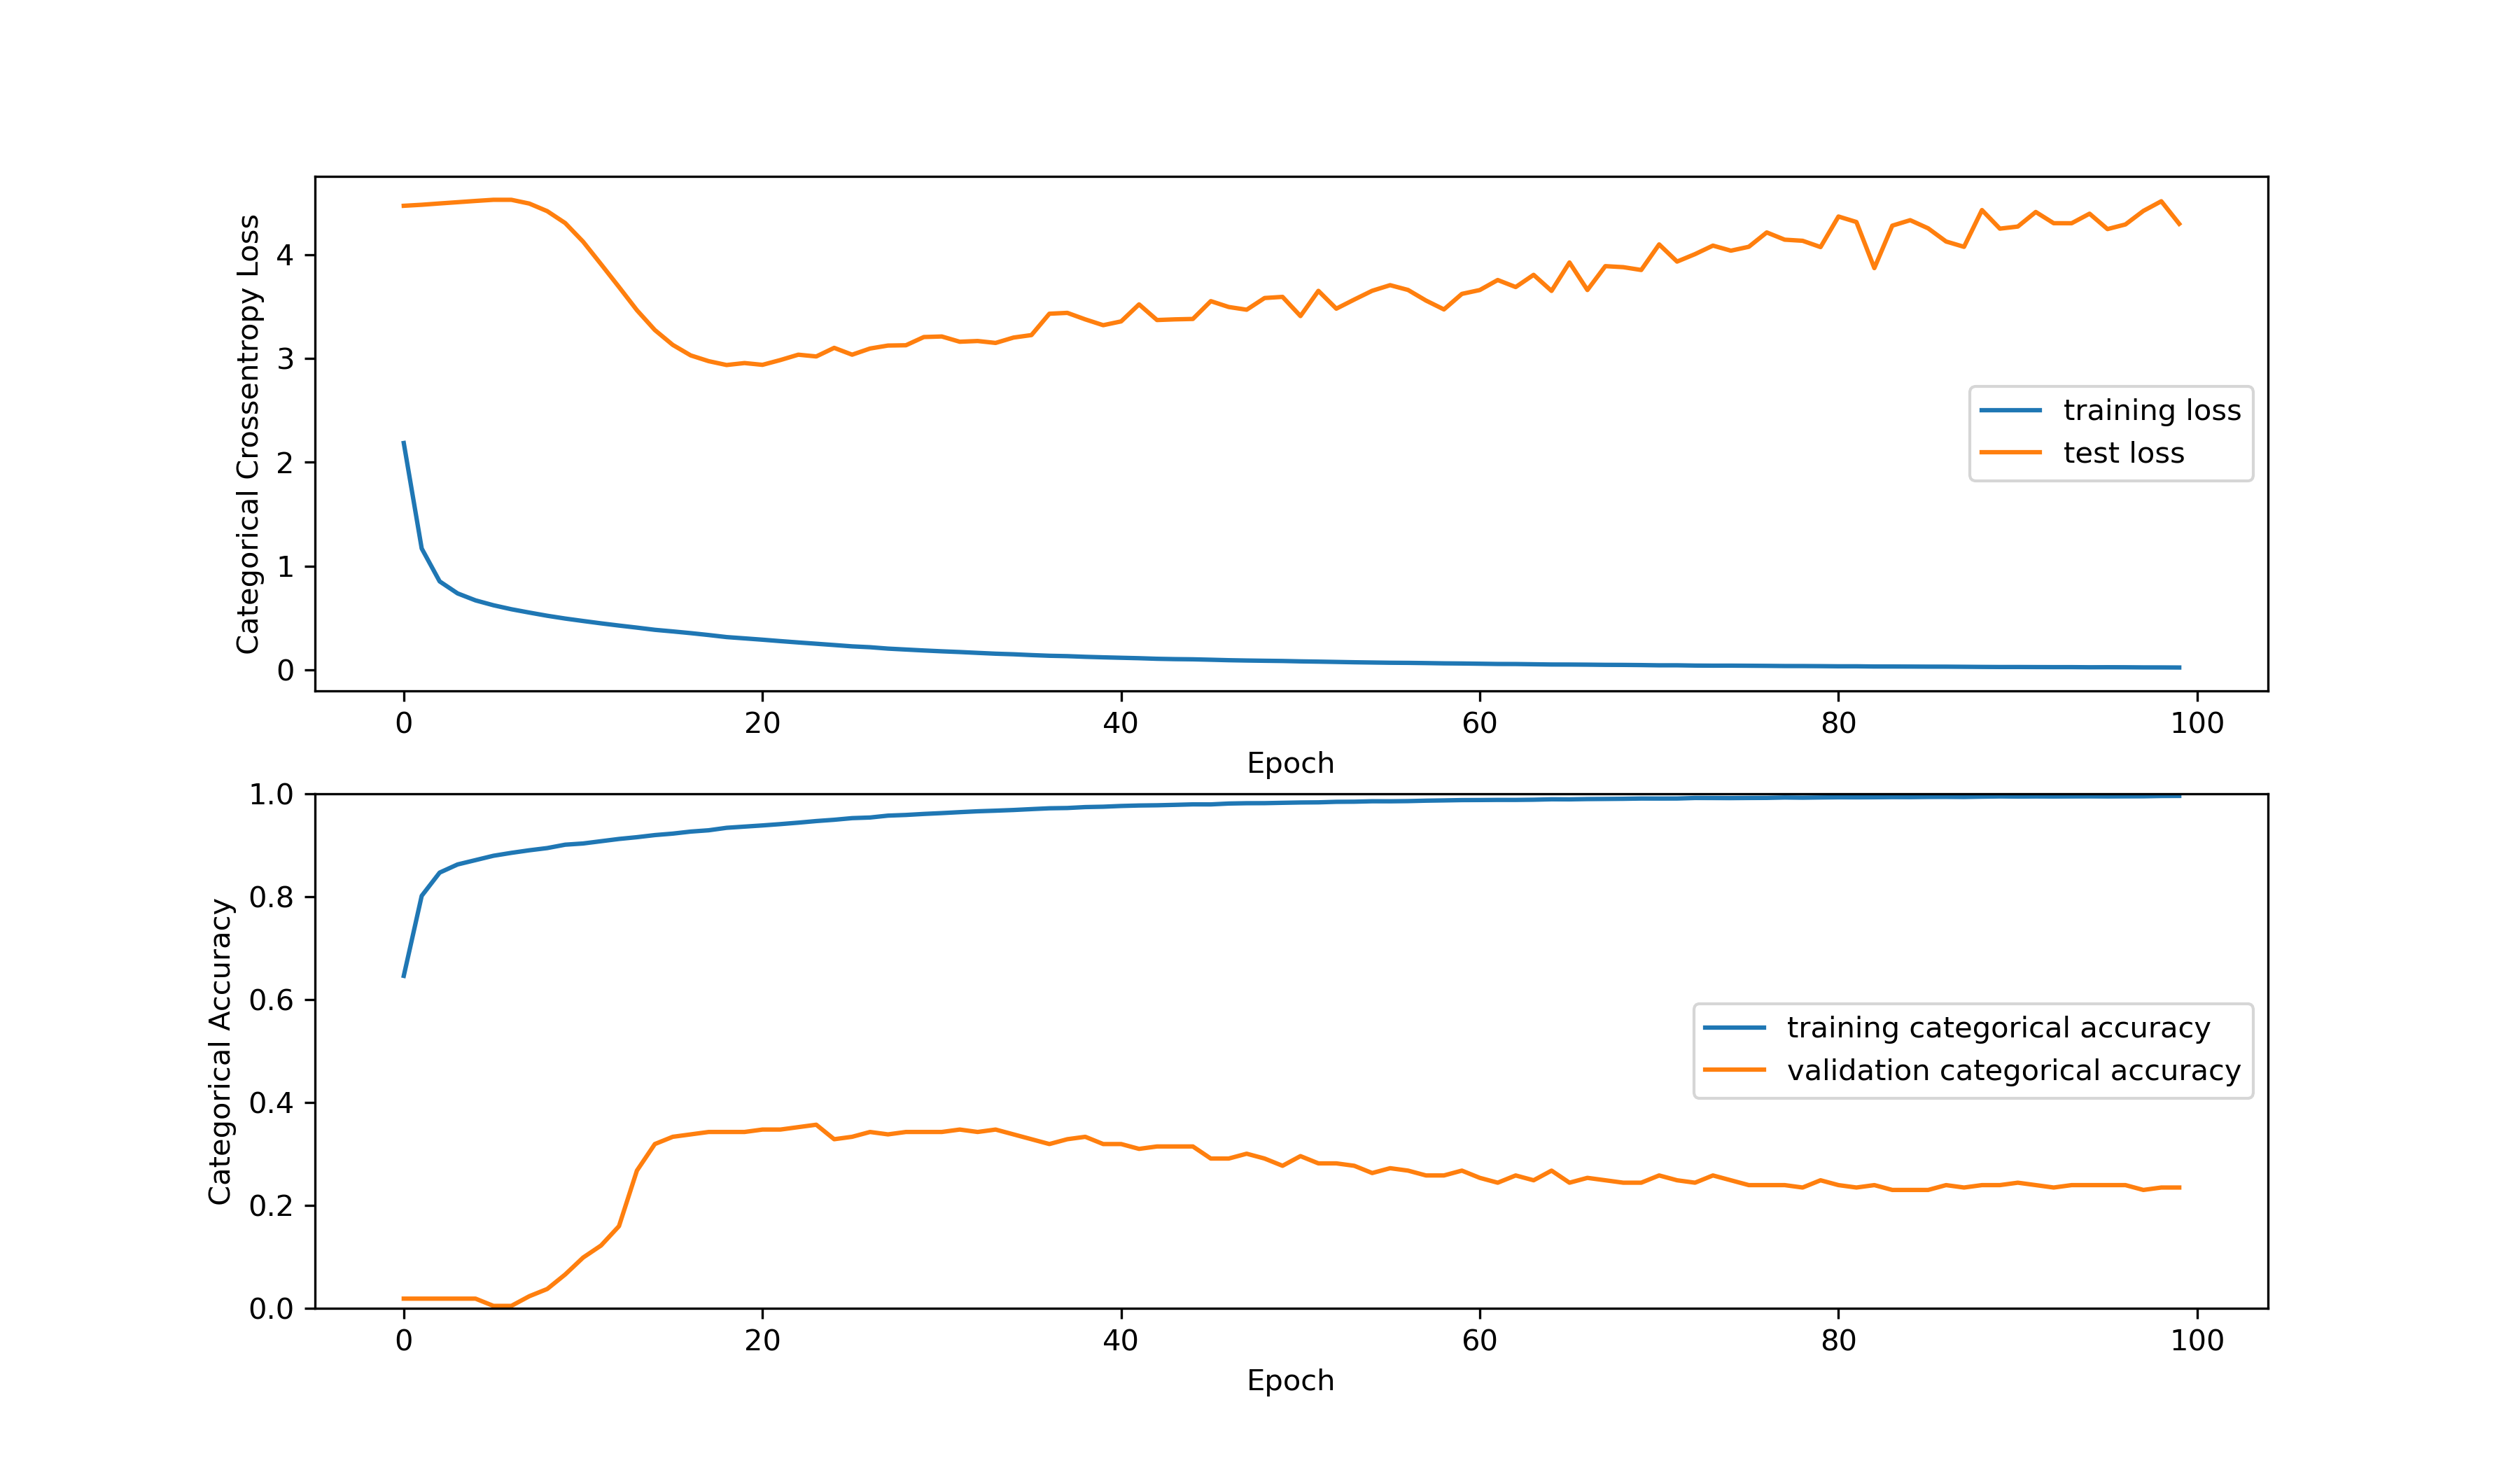
\includegraphics[width=\textwidth]{Figures/overfit.png}
    \caption{Overfit of a CBAM model}
    \label{fig:overfit}
\end{figure}


\subsection{Domain gap}

% domain gap between experimental and simulated - learning the difference is hard!

\section{}
